%; whizzy chapter
% -initex iniptex -latex platex -format platex -bibtex jbibtex -fmt fmt
% $B0J>e(B whizzytex $B$r;HMQ$9$k>l9g$N@_Dj!#(B

%     Kansai Debian Meeting resources
%     Copyright (C) 2007 Takaya Yamashita
%     Thank you for Tokyo Debian Meeting resources

%     This program is free software; you can redistribute it and/or modify
%     it under the terms of the GNU General Public License as published by
%     the Free Software Foundation; either version 2 of the License, or
%     (at your option) any later version.

%     This program is distributed in the hope that it will be useful,
%     but WITHOUT ANY WARRANTY; without even the implied warranty of
%     MERCHANTABILITY or FITNESS FOR A PARTICULAR PURPOSE.  See the
%     GNU General Public License for more details.

%     You should have received a copy of the GNU General Public License
%     along with this program; if not, write to the Free Software
%     Foundation, Inc., 51 Franklin St, Fifth Floor, Boston, MA  02110-1301 USA

%  preview (shell-command (concat "evince " (replace-regexp-in-string "tex$" "pdf"(buffer-file-name)) "&"))
% $B2hA|%U%!%$%k$r=hM}$9$k$?$a$K$O(Bebb$B$rMxMQ$7$F(Bboundingbox$B$r:n@.!#(B
%(shell-command "cd image200708; ebb *.png")

%%$B$3$3$+$i%X%C%@3+;O!#(B

\documentclass[mingoth,a4paper]{jsarticle}
\usepackage{kansaimonthlyreport}
\usepackage[dvips]{xy}

% $BF|IU$rDj5A$9$k!"Kh7nJQ$o$j$^$9!#(B
\newcommand{\debmtgyear}{2012}
\newcommand{\debmtgdate}{26}
\newcommand{\debmtgmonth}{8}
\newcommand{\debmtgnumber}{63}

\begin{document}

\begin{titlepage}

% $BKh7nJQ99$9$kItJ,!"K\J8$NKvHx$b=$@5$9$k$3$H$r$o$9$l$:$K(B

 $BBh(B\debmtgnumber{}$B2s(B $B4X@>(B Debian $BJY6/2q;qNA(B

\vspace{2cm}

\begin{center}
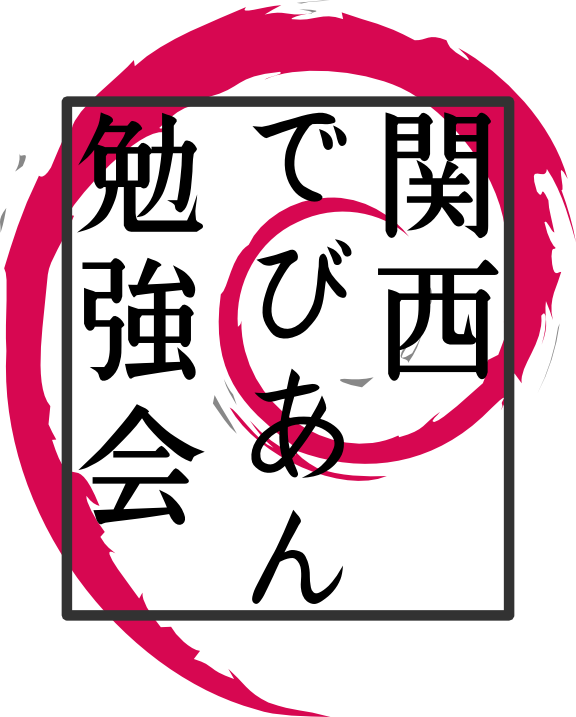
\includegraphics{image200802/kansaidebianlogo.png}
\end{center}

\begin{flushright}
\hfill{}$B4X@>(B Debian $BJY6/2qC4Ev<T(B $B:4!9LZ!&ARI_!&$N$,$?!&$+$o$@(B \\
\hfill{}\debmtgyear{}$BG/(B\debmtgmonth{}$B7n(B\debmtgdate{}$BF|(B
\end{flushright}

\thispagestyle{empty}
\end{titlepage}

\dancersection{Introduction}{Debian JP}

 $B4X@>(BDebian$BJY6/2q$O(BDebian GNU/Linux$B$N$5$^$6$^$J%H%T%C%/(B
 ($B?7$7$$%Q%C%1!<%8!"(BDebian$BFCM-$N5!G=$N;EAH!"(BDebian$B3&7($G5/$3$C$?=PMh;v!"(B
 $B$J$I$J$I!K$K$D$$$FOC$79g$&2q$G$9!#(B

 $BL\E*$H$7$F<!$N;0$D$r9M$($F$$$^$9!#(B
 \begin{itemize}
  \item ML$B$d7G<(HD$G$O$J$/!"D>@\4i$r9g$o$;$k;v$G$N>pJs8r49$NB%?J(B
  \item $BDj4|E*$K=8$^$l$k>l=j(B
  \item $B;qNA$N:n@.(B
 \end{itemize}

 $B$=$l$G$O!"3Z$7$$0l;~$r$*3Z$7$_2<$5$$!#(B

\newpage

\begin{minipage}[b]{0.2\hsize}
 {\rotatebox{90}{\fontsize{80}{80}
{\gt $B4X@>(B Debian $BJY6/2q(B}}}
\end{minipage}
\begin{minipage}[b]{0.8\hsize}
\hrule
\vspace{2mm}
\hrule
\setcounter{tocdepth}{1}
\tableofcontents
\vspace{2mm}
\hrule
\end{minipage}

\dancersection{$B:G6a$N(BDebian$B4X78$N%$%Y%s%HJs9p(B}{Debian JP}

\subsection{$BBh(B 62 $B2s4X@>(B Debian $BJY6/2q(B@OSC012Kansai@Kyoto}

62 $B2sL\$N4X@>(B Debian $BJY6/2q$O:#7n(B 3 $BF|!"(B4$BF|$K5~ET%j%5!<%A%Q!<%/$G9T$J$o$l$?%*!<%W%s%=!<%9%+%s%U%!%l%s%9$G9T$J$$$^$7$?!#(B

$B%;%_%J!<$G$O!V(BDebian 7.0  ``Wheezy'' frozen$B!W$HBj$7$F(B 6 $B7n$K%U%j!<%:$5$l$?<!4|%j%j!<%98uJd$N(B Debian 7.0 ``Wheezy'' $B$N>R2p$r9T$J$$$^$7$?!#(B
$B%V!<%9$NJ}$K$bB?$/$NJ}$KN)$A4s$C$FD:$-!"Cf$G$b(B Debian T $B%7%c%D$OBgJQ9%I>$G$7$?!#(B

\subsection{$BBh(B 91 $B2sEl5~%(%j%"(B Debian $BJY6/2q(B}
91 $B2sL\$NEl5~%(%j%"(B Debian $BJY6/2q$O(B 8 $B7n(B 2 $BF|$K3+:E$5$l$^$7$?!#(B

DebConf 12 $B;22CJs9p!"7n4)(B Debhelper$B!"%=%U%H3+H/0J30$N4JC1(B Debian contribution($B%I%i%U%HHG(B!)$B!"(BDebian $B$G$N(B C++11 $B3+H/4D6-(B
$B$H$$$C$?FbMF$G$7$?!#(B

Debian contribution $B$G$O%=%U%H3+H/0J30$NMM!9$J(B Debian $B$X$N9W8%J}K!$,>R2p$5$l$F$$$^$9!#(B
$B%Q%C%1!<%8%a%s%F%J%s%9$OFq$7$$$1$l$I2?$+9W8%$7$?$$$H;W$o$l$F$$$kJ}$O;29M$K$7$F2?$+$d$C$F$_$h$&$H;W$o$l$k$3$H$+$i;O$a$F$_$F$O$$$+$,$G$7$g$&$+!#(B

\dancersection{$B;vA02]Bj(B}{Debian JP}

$B:#2s$O0J2<$N2]Bj$r=PBj$7$^$7$?(B.
\begin{screen}
  \begin{enumerate}
  \item MIT$BHG(BKerberos$B$G%5!<%S%9$KI,MW$H$J$k%W%m%;%9L>$H!"$=$N%W%m%;%9$,;HMQ$9$k%]!<%H$r(B 2 $B$D0J>e5s$2$F$/$@$5$$!#(B

  \item DebConf12$B$G$N;qNA$rM==,$7$F$*$$$F$/$@$5$$!#(B\\
   \url{http://penta.debconf.org/dc12_schedule/events/894.en.html}

  \end{enumerate}
\end{screen}

$B;22C<T$N3'$5$s$N2rEz$O0J2<$NDL$j$G$9!#(B

\begin{prework}{ $B$H$_!<(B }
  \begin{enumerate}
  \item $B$^$C$?$/$o$+$j$^$;$s$,!";22C$7$FJY6/$7$?$$$H$*$b$$$^$9!#(B
  \end{enumerate}
\end{prework}

\begin{prework}{ $B$+$o$@$F$D$?$m$&(B }
  \begin{enumerate}
  \item sid $B4D6-$G(B krb5-\{admin-server,kdc\} $B$r%$%s%9%H!<%k$7$F3NG'!#(B
    \begin{itemize}
    \item krb5kdc 88/udp 750/udp
    \item kadmind 464/udp 464/tcp 749/tcp
    \end{itemize}
  \item $B8+$F$*$-$^$9!#(B
  \end{enumerate}
\end{prework}

\begin{prework}{ okumura.d }
  \begin{enumerate}
  \item kadmind $B%W%m%;%9!#(Btcp$B5Z$S(Budp$B%]!<%HHV9f$O(B88,749.\\
    \#750(Kerberos RFile)$B$O(BWindows$B8BDj(B..?
  \end{enumerate}
\end{prework}

\begin{prework}{ $B:4!9LZMNJ?(B }
  \begin{enumerate}
  \item
    \begin{itemize}
    \item process
      \begin{itemize}
      \item krb5-admin-server
      \item krb5-kdc
      \end{itemize}
    \item port
      \begin{itemize}
      \item 88/udp, 754/tcp, 760/tcp
      \end{itemize}
    \end{itemize}
  \item $B8+$F$*$-$^$9$k!#(B
  \end{enumerate}
\end{prework}

\begin{prework}{ $BLZ2<(B }
  \begin{enumerate}
  \item $B%1%k%Y%m%9G'>Z$G$O!"!V(BKDC$B!J(BKey Distribution Center$B!K!W$H8F$P$l$k%5!<%P!<$rMQ0U$7!"$=$3$KG'>Z>pJs$r0l854IM}!#(B\\
    $B"*%f!<%6!<$,J#?t%5!<%P!<$rMxMQ$9$k>l9g!"0lEYG'>Z$r<u$1$k$@$1$G!"$[$+$N%5!<%P!<$X$b%"%/%;%9$G$-$k$h$&$K$J$j!"2?EY$b%m%0%$%s$9$kI,MW$,$J$/$J$k!#(B
    \begin{enumerate}
    \item $B%5!<%S%9$KI,MW$H$J$k%W%m%;%9L>(B
      \begin{itemize}
      \item krb5kdc$B!J(BKerberos $B%5!<%P!<!K(B
      \item kadmin$B!J(Bkadmin $B%f!<%F%#%j%F%#!K(B
      \item krb524$B!J!)ITL@!K(B
      \end{itemize}
    \item $B%5!<%S%9$KI,MW$H$J$k%W%m%;%9L>(B
      \begin{itemize}
      \item $B$9$_$^$;$s!#;~4V$,$J$/D4$Y$i$l$F$$$^$;$s!#(B
      \end{itemize}
    \end{enumerate}
  \item $B;~4V$N5v$98B$j8+$F$*$-$^$9!#(B
  \end{enumerate}
\end{prework}

\begin{prework}{ yyatsuo }
  \begin{enumerate}
  \item $BJY6/$7$F$*$-$^$9!#(B
  \item $BJY6/$7$F$*$-$^$9!#(B
  \end{enumerate}
\end{prework}

\begin{prework}{ 0xBCD1BC92 }
  \begin{enumerate}
  \item $B%$%s%9%H!<%k$7$?$i$o$+$k$N$+$b$7$l$J$$$,!"(B/etc/init.d$B$N%W%m%;%9$r%-%C%/$9$kL>A0$G$*Cc$rBy$7$F$*$/!#$7$?$N(B/etc/serivces$B$HO"F0$7$F$$$k$+$b$7$l$:!#(B
    \begin{itemize}
    \item krb5-admin-server
    \item krb5-kdc
    \end{itemize}
    /etc/services $B$+$i=&$C$?$+$i@52r$@$H;W$&!#(B
    \begin{itemize}
    \item 88/udp
    \item 754/tcp         krb5\_prop hprop
    \item 760/tcp         kreg
    \end{itemize}
  \item $B;qNA$O!";E;v$N4V$K$K$i$s$G$*$-$^$9!#(B
  \end{enumerate}
\end{prework}

\begin{prework}{ $B@>;3OB9-(B }
  \begin{enumerate}
  \item kadmind $B$G(B TCP $B$N(B 749 $B$H(B 464
  \end{enumerate}
\end{prework}

\begin{prework}{ $B0BItIp;V(B }
  \begin{enumerate}
  \item $B%W%m%;%9L>(B: krb5kdc (KDC)\\
    $B;HMQ$9$k%]!<%HHV9f(B: 88 $B$*$h$S(B 750
  \end{enumerate}
\end{prework}

\begin{prework}{ $B2,!!BgJe(B }
  \begin{enumerate}
  \item $B$I$3$rD4$Y$l$P$$$$$N$+$o$+$i$J$$!#(BKerberos$BG'>Z$,$I$&$$$&$b$N$+$O%0%0$k$3$H$G$o$+$C$?!#$b$&>/$7%/%m!<%j%s%0$7$F$_$k!#(B
  \end{enumerate}
\end{prework}

\begin{prework}{ $B;3>k$N9q$N=;?M(B $B5WJ]Gn(B }
  \begin{enumerate}
  \item squeeze $B4D6-$G(B MIT Kerberos $B$rF0$+$7$F!"%5!<%S%9$,;H$&%]!<%HHV9f$r<!$N$h$&$KD4$Y$^$7$?!#(B
    \begin{commandline}
lsof -p `pgrep krb5kdc`
lsof -p `pgrep kadmind`
    \end{commandline}
    \begin{itemize}
    \item $B%W%m%;%9L>(B: krb5kdc
    \item $B%]!<%HHV9f(B: 88/udp 750/udp
    \item $B%W%m%;%9L>(B: kadmind
    \item $B%]!<%HHV9f(B: 749/tcp 464/tcp 464/udp
    \end{itemize}
  \item $B$O$$!#EvF|$^$G$K$O2?$H$+!#(B
  \end{enumerate}
\end{prework}

\begin{prework}{ lurdan }
  \begin{enumerate}
  \item $BB3$-$O(B We\^h\^h $B%;%C%7%g%s$G!*(B
  \item $B0l1~%S%G%*8+$^$7$?!#Fq$7$$$G$9!#(B
  \end{enumerate}
\end{prework}

\clearpage

\dancersection{Debian $B$G$O$8$a$k(B Kerberos $BG'>Z(B}{$BARI_(B $B8g(B}

\subsection{$B;vA02]Bj$N3NG'(B}

$B:#2s$N;vA02]Bj$O!"!V(BMIT $BHG(B Kerberos $B$N%5!<%S%9$r9=@.$9$k%W%m%;%9$H!"$=$N%W%m%;%9$,;HMQ$9$k%]!<%H$r(B 2 $B$D0J>e5s$2$F$/$@$5$$!W$G$7$?!#(B

$B@52r$O!"(BMIT $BHG(B Kerberos $B$N4IM}%,%$%I(B\footnote{\url{http://web.mit.edu/kerberos/krb5-1.10/krb5-1.10.3/doc/krb5-admin.html\#Configuring-Your-Firewall-to-Work-With-Kerberos-V5}}$B$r;2>H$7$F$/$@$5$$!#0l1~!"(BKerberos $B2=$5$l$?%5!<%S%9$J$I$r>J$$$?LOHO2sEzNc$O2<5-$NDL$j$G$9!#(B

\begin{description}
\item [krb5kdc] 88/tcp,udp
\item [kadmind] 749/tcp
\item [kpropd] 754/tcp
\end{description}

\subsection{kerberos $B$H$O(B}

1980 $BG/Be$K(B MIT $B$N%"%F%J%W%m%8%'%/%H(B\footnote{$B6=L#$N$"$kJ}$O!"!V(BMIT$B%"%F%J%W%m%8%'%/%H$N$9$Y$F!W$H$$$&=q@R$rFI$`$H3Z$7$a$k;W$$$^$9(B}$B$G(B (X Window System $B$J$I$H$H$b$K(B) $B3+H/$5$l$?!"%*!<%W%s$J%M%C%H%o!<%/$K$*$1$kG'>Z%7%9%F%`$G$9!#$b$H$b$H!"(BMIT $B$N%*!<%W%s%-%c%s%Q%9$K$*$1$k2]Bj$r2r7h$9$k$?$a$K3+H/$5$l$F$$$k$?$a!"%;%-%e%"$G$O$J$$J,;64D6-$G$NF0:n$,A0Ds$K$J$C$F$$$kB>!"%7%s%0%k!&%5%$%s%*%s$b%5%]!<%H$5$l$F$$$^$9!#(B

$B3+H/=i4|$K8x3+$9$k$&$($GJF9q$N0E9f@/:v(B ($BM"=P6X;_(B) $B$r2sHr$9$kI,MW$,$"$C$?$?$a!"(Bkerberos $B$K$OJ#?t$N<BAu$,$"$j$^$9!#$?$@!"8=:_$G$OFC$KLdBj$J$/(B MIT $B$N<BAu$rMxMQ$9$k$3$H$,$G$-$^$9$N$G!"JL<BAu$N$3$H$O$R$H$^$:$*$$$F$*$-$^$7$g$&!#6=L#$N$"$kJ}$O(B kth $B$H$+(B heimdal $B$H$+$G%0%0$C$F$_$F$/$@$5$$!#(B

$B%P!<%8%g%s(B5$B0J9_$G$O!"(Bkerberos $B%W%m%H%3%k$H$7$F(B RFC $B$,H/9T$5$l$F$$$^$9(B\footnote{http://www.ipa.go.jp/security/rfc/RFC.html\#10}$B!#$^$?!"(BWindows2000 $B0J9_$N(B AD $BG'>Z$G$bMxMQ$5$l$F$$$k$N$G!"5$IU$+$J$$$&$A$K;H$C$F$$$?!"$H$$$&J}$b$$$k$+$b$7$l$^$;$s!#(B

\subsubsection{kerberos $B$NMQ8l(B}

\begin{description}
  \item [$B%l%k%`(B] $B$"$k(B KDC $B$,4IM}BP>]$H$9$k%M%C%H%o!<%/$NHO0O$G$9!#(BDNS $B%I%a%$%s$HBP1~$5$;$k$3$H$,B?$$$h$&$G$9!#(BActiveDirectory $BE*$K$O%U%)%l%9%H$K$J$j$^$9!#(B
  \item [$B%W%j%s%7%Q%k(B] kerberos $B$N4IM}BP>]$H$J$k$"$i$f$k8DJL$NMWAG$G$9!#%f!<%6!"%[%9%H!"%5!<%S%9$J$I$,4^$^$l$^$9!#<!$N=q<0$NJ8;zNs$GI=8=$5$l$^$9!#!VL>A0(B/$B<1JL;R(B@$B%l%k%`!W(B

  \item [$B80H/9T6I(B (KDC: Key Distribution Center)] kerberos $B$N%-%b$H$J$k%5!<%S%9$G$9!#4IM}%l%k%`$K=jB0$7$F$$$kA4%W%j%s%7%Q%k$NHkL)80$rJ];}$7$F$*$j!"%f!<%6$NG'>Z(B (AS) $B$H!"%A%1%C%H$NH/9T(B (TGS) $B$r9T$$$^$9!#(B

  \item [$B%A%1%C%H(B] $B%f!<%6$+$i$NMW5a$K1~$8$F80H/9T6I$G@8@.$5$l$k!"4|8B$D$-$NG'>Z%G!<%?$G!"6&M-80$G0E9f2=$5$l$F$$$^$9!#(B

  \item [TGT (Ticket Granting Ticket)] $B%f!<%6$,G'>Z$K@.8y$7$?>l9g$KH/9T$5$l$k%A%1%C%H$G!"FbIt$K0l;~E*$J%;%C%7%g%s80$rJ];}$7$F$$$^$9!#$3$l$r;}$C$F$$$k%f!<%6$N$_!"%5!<%S%9%A%1%C%H$NH/9T$,5v2D$5$l$^$9!#(B
  \item [$B80%F!<%V%k(B (Key Table)] Kerberos $BG'>Z$r<u$1$k%5!<%S%9$GI,MW$H$J$k!"%W%j%s%7%Q%k$H80$N0lMw%U%!%$%k$G$9!#(BKDC $B>e$G%[%9%H%W%j%s%7%Q%k$H%5!<%S%9%W%j%s%7%Q%k$r:n@.$7!"$=$l$r%U%!%$%k$K=PNO$7$F$+$i3:Ev$N%[%9%H$K%3%T!<$9$kI,MW$,$"$j$^$9!#(B

\end{description}

Kerberos $B$N;EAH$_$dF0:n$N>\:Y$K$D$$$F$O!"!V(B3$BJ,4V(B NetWorking$B!W$H$$$&%5%$%H(B\footnote{\url{http://www5e.biglobe.ne.jp/\%257Eaji/3min/ex/sup04.html}}$B$,8l$j8}$b7Z$/!"$o$+$j$d$9$$$H;W$$$^$9$N$G0lEYFI$s$G$_$F$/$@$5$$!#(B20 $BJ,$[$I$GFI$a$^$9!#(B

\subsection{$B9=@.$N;vA0=`Hw(B}
kerberos $B$G$O!"%[%9%H$NL>A02r7h$,$G$-$k$3$H!";~9o$,F14|$7$F$$$k$3$H!"$,A0Ds>r7o$H$7$FI,MW$K$J$j$^$9!#$A$g$C$HLLE]$G$9$,!"3NG'$7$F$*$$$F$/$@$5$$!#(B

$BE,Ev$J2>A[2=5!G=$r;H$C$?<B83$G$"$l$P!"L>A02r7h$O(B dnsmasq $B%Q%C%1!<%8$rF3F~$7$F(B /etc/hosts $B$K$5$C$/$j=q$/$N$,$*<j7Z$GJXMx$+$H;W$$$^$9!#(B

\subsection{$BG'>Z%5!<%P$N9=@.(B}

$B%f!<%6G'>Z$N4QE@$G$O!"(Bkerberos $B$O%"%+%&%s%HL>$H%Q%9%o!<%I$NAH$@$1$r07$$$^$9$N$G!"%[!<%`%G%#%l%/%H%j$d%7%'%k$,@_Dj$G$-$^$;$s!#$=$3$G:#2s$O!"(Bopenldap $B$r%"%+%&%s%H$N%a%?%G!<%?$rJ]4I$9$k%G!<%?%Y!<%9$H$7$F;HMQ$7$^$9!#(B
openldap $B$N9=C[$H@_Dj$K$D$$$F$O!":4!9LZ$5$s$K$h$kA02s$N4X@>(B Debian $BJY6/2q;qNA$+!"F1$8$/:4!9LZ$5$s$K$h$k<!2s$N(B Debian $BJY6/2q;qNA$r;29M$K$7$F$/$@$5$$!#$3$3$G$O!"$9$G$K@_Dj$,40N;$7$F$$$k$b$N$H$7$F?J$a$^$9!#(B

/etc/passwd $B$H(B /etc/shadow $BAjEv$N%G!<%?$rJ];}$9$k$b$N$H$7$F!"%*%V%8%'%/%H%/%i%9$O(B posixAccount $B$H(B shadowAccount $B$rMxMQ$7$^$9!#$?$@$7!"<B:]$K$O(B shadowAccount $B$NB0@-$OMxMQ$7$^$;$s!#(B
/etc/shadow $BAjEv$N<B%G!<%?$O(B kerberos $B$G<h$j07$&$N$G$9$,!"$=$l$O(B OS $B$+$i(B shadow $B>pJs$H$7$F8+$($k$o$1$G$O$J$$$N$G!"%U%'%$%/$N%"%/%;%9@h$H$$$&0LCVIU$1$G$9!#(B

openldap $B$H(B kerberos $B$O(B 1 $BBf$N%5!<%P$KF15o$5$;$k$H$$$&A[Dj$G!"$^$:$O(B kerberos $B%5!<%S%9MQ$N%Q%C%1!<%8$r%$%s%9%H!<%k$7$F$_$^$7$g$&!#(B

\begin{commandline}
unset DEBIAN_FRONTEND $B"((Bpbuilder $B$G<B83$7$F$$$k>l9g(B
apt-get install lv vim
apt-get install krb5-kdc krb5-admin-server
\end{commandline}

krb5-kdc $B$,80H/9T6I$G!"(Bkrb5-admin-server $B$,%"%+%&%s%H>pJs$N4IM}%W%m%H%3%k$r=hM}$7$^$9!#(Bdebconf $B$,$$$/$D$+<ALd$r$7$F$/$k$H;W$$$^$9$,!"!V(BYes/No $B$N<ALd$OA4$F%G%U%)%k%HDL$j!W!"!V(BDefault Kerberos version 5 realm$B!W$K$OL>A02r7h$G;H$C$F$$$k%I%a%$%sL>!"!V%5!<%P%"%I%l%9!W$K$OL>A02r7h$G$-$k%[%9%HL>!"$r$=$l$>$lF~NO$7$F$/$@$5$$!#(B

kerberos $BA4HL$N@_Dj%U%!%$%k$O!"(B/etc/krb5.conf $B$K$J$j$^$9!#%$%s%9%H!<%k;~$K(B debconf $B$,<+F0$G@8@.$7$F$/$l$k$N$G$9$,!"JQ99$,ITB-$7$F$$$k$N$G<jJT=8$,I,MW$G$9!#(B

\begin{commandline}
vi /etc/krb5.conf
\end{commandline}

\begin{itemize}
\item ($BI,?\(B) [domain\_realm]$B$K%I%a%$%s$N@_Dj$rDI2C(B
\item ($B%*%W%7%g%s(B) [realms] $B$+$iITMW$J$b$N$r>C$9(B
\item ($B%*%W%7%g%s(B) [domain\_realm] $B$+$iITMW$J$b$N$r>C$9(B
\end{itemize}

$B@_Dj%U%!%$%k$NJT=8$,=*$o$C$?$i!"(Bkerberos $B$N%G!<%?%Y!<%9$r=i4|2=$7$^$7$g$&!#(Bdebian $B$K$O!"$3$N$?$a$N$A$g$C$H$7$?%9%/%j%W%H$,IUB0$7$F$$$^$9!#(B

\begin{commandline}
krb5_newrealm
\end{commandline}

root/admin $B$N%Q%9%o!<%I$r5a$a$i$l$^$9$N$G!"F~NO$7$F$/$@$5$$!#$3$l$rK:$l$k$H$I$&$K$b$J$i$J$/$J$k$N$G!"K:$l$J$$$h$&$KJLES$7$C$+$j4IM}$7$F$*$-$^$7$g$&!#(B
$B$3$NCJ3,$G!"6u$N%G!<%?%Y!<%9$,:n@.$5$l!"3F<o%W%j%s%7%Q%k$NEPO?$dJQ99$,$G$-$k$h$&$K$J$C$F$$$^$9!#(B

\subsection{$B%G!<%?$NEPO?(B}

\subsubsection{kadmin.local}

kerberos $B$N4IM}:n6H$K;H$&%3%^%s%I$K$O!"(Bkadmin$B!"(Bkadmin.local$B!"(Bkdb5\_util $B$J$I$,$"$j$^$9!#$3$N$&$A!"(Bkadmin.local $B$O4IM}%5!<%P>e$G$N$_MxMQ$G$-$k$b$N$G$9!#(B
kadmin $B$r;H$&$K$O(B kerberos $B$G$N%f!<%6G'>Z$r%Q%9$9$kI,MW$,$"$k!"$D$^$j%W%j%s%7%Q%k$rEPO?$7$F$+$i$G$J$$$H;H$($J$$$N$G!":G=i$O(B kadmin.local $B$G4IM}:n6H$r9T$$$^$9!#(B

kadmin.local $B$r<B9T$9$k$H!"%W%m%s%W%H$,=PNO$5$l$F4IM}%3%^%s%I$NF~NOBT$A$K$J$j$^$9!#(B'?' $B$G%3%^%s%I$N%j%9%H$,I=<($5$l$^$9$N$GD/$a$F$_$^$7$g$&!#(B

\begin{commandline}
kadmin.local:  ?
Available kadmin.local requests:

add_principal, addprinc, ank
                         Add principal
delete_principal, delprinc
                         Delete principal
modify_principal, modprinc
                         Modify principal
rename_principal, renprinc
                         Rename principal
change_password, cpw     Change password
get_principal, getprinc  Get principal
list_principals, listprincs, get_principals, getprincs
                         List principals
add_policy, addpol       Add policy
modify_policy, modpol    Modify policy
delete_policy, delpol    Delete policy
get_policy, getpol       Get policy
list_policies, listpols, get_policies, getpols
                         List policies
get_privs, getprivs      Get privileges
ktadd, xst               Add entry(s) to a keytab
ktremove, ktrem          Remove entry(s) from a keytab
lock                     Lock database exclusively (use with extreme caution!)
unlock                   Release exclusive database lock
purgekeys                Purge previously retained old keys from a principal
get_strings, getstrs     Show string attributes on a principal
set_string, setstr       Set a string attribute on a principal
del_string, delstr       Delete a string attribute on a principal
list_requests, lr, ?     List available requests.
quit, exit, q            Exit program.
\end{commandline}

$B$H$j$"$($:!"$3$3$G$O%W%j%s%7%Q%k$NEPO?$H3NG'$@$1$6$C$/$j8+$F$_$k$3$H$K$7$^$9!#(B

\subsubsection{$B%f!<%6%W%j%s%7%Q%k(B}

$B%f!<%6$NDI2C$O4JC1$G!"%W%j%s%7%Q%k$NL>A0$H$7$F%f!<%6L>$r;XDj$9$k$@$1$G$9!#(B

\begin{commandline}
addprinc kdmtest
\end{commandline}

$B%Q%9%o!<%I$r5a$a$i$l$^$9$N$G!"F~NO$7$F$/$@$5$$!#(B

\subsubsection{$B%[%9%H%W%j%s%7%Q%k(B}

$B%[%9%H$rDI2C$9$k>l9g$O!"%W%j%s%7%Q%k$NL>A0$H$7$F(B host$B!"<1JL;R$H$7$F$=$N%[%9%H$N(B FQDN $B$r;XDj$7$^$9!#(B
$B$^$?!"%[%9%H$N>l9g$O%Q%9%o!<%I$r?M4V$,F~NO$9$k$3$H$O$J$$$N$G!"<jF~NO$G$J$/%i%s%@%`$J$b$N$r<+F0@8@.$5$;$^$9!#(B

\begin{commandline}
addprinc -randkey host/dandelion.localdomain
\end{commandline}

\subsubsection{$B%5!<%S%9%W%j%s%7%Q%k(B}

$B%5!<%S%9$rDI2C$9$k>l9g$O!"%W%j%s%7%Q%k$NL>A0$H$7$F%5!<%S%9L>!"<1JL;R$H$7$F%5!<%S%9$rDs6!$9$k%[%9%H$N(B FQDN $B$r;XDj$7$^$9!#(B

\begin{commandline}
addprinc -randkey ldap/dandelion.localdomain
\end{commandline}

\subsubsection{$BEPO?%G!<%?$N3NG'(B}

listprincs $B%3%^%s%I$G!"EPO?$5$l$F$$$k%W%j%s%7%Q%k$N0lMw$rI=<($9$k$3$H$,$G$-$^$9!#=i4|>uBV$G$O!"<!$N$h$&$K$J$C$F$$$k$H;W$$$^$9!#(B

\begin{commandline}
K/M@YOUR.REALM
kadmin/admin@YOUR.REALM
kadmin/changepw@YOUR.REALM
kadmin/yourhost.localdomain@YOUR.REALM
krbtgt/YOUR.REALM@YOUR.REALM
\end{commandline}

\subsubsection{$B80%F!<%V%k%U%!%$%k(B (ktab) $B$N@8@.(B}

$B%W%j%s%7%Q%kL>$r;XDj$7$F(B ktadd $B%3%^%s%I$r<B9T$9$k$3$H$G!"80%F!<%V%k$r:n@.(B/$B99?7$9$k$3$H$,$G$-$^$9!#(B
$BFCDj%5!<%S%9%[%9%HMQ$N80%F!<%V%k%U%!%$%k$O!"LLE]$G$9$,JLESE>Aw$7$F$*$/I,MW$,$"$j$^$9$N$G!"K:$l$J$$$h$&$KCm0U$7$^$7$g$&!#(B

\subsection{$B%/%i%$%"%s%H$N9=@.(B}

NSS $B$K;2>H$5$;$k%i%$%V%i%j$K$O!"$$$/$D$+$NA*Br;h$,B8:_$7$^$9!#(B

\begin{table}[htb]
  \begin{tabular}{lcccr}
    $B%/%i%$%"%s%H(B & LDAP & Kerberos & TLS & $BHw9M(B \\
    lib(nss/pam)-ldap & $B!{(B & $B!_(B & $BL$BP1~(B & $B8E$$$,B?5!G=(B \\
    lib(nss/pam)-ldapd & $B!{(B & $B!_(B & $BBP1~(B & squeeze $B0J9_$N?d>)!#$^$@H/E8ES>e(B \\
    libpam-krb5 & $B!_(B & $B!{(B & $B!](B & \\
    sssd & $B!{(B & $B!{(B & $BI,?\(B & RedHat $B$,(B FreeIPA $B$N$?$a$K3+H/$7$F$$$k!#$^$@H/E8ES>e(B \\
  \end{tabular}
\end{table}

Debian $BE*$K$O!":#2s$N9=@.$G$"$l$P(B libnss-ldapd + libpam-krb5 $B$,K\L?$H$$$&$3$H$K$J$k$N$+$bCN$l$^$;$s$,!"$3$3$G$O;n$7$K(B sssd $B$r;H$C$F$_$k$3$H$K$7$^$9!#(B

sssd $B$O!"(BRedHat $B$,$h$/$d$k!"$"$l$3$l0l=o$/$?$K$^$H$a$k7O$N:F<BAu$N0l$D$G!">e5-$N(B ldap/krb $B8~$1$N%/%i%$%"%s%H5!G=$NB>!"(BNSCD $B$N5!G=$b;}$C$F$$$^$9!#(B

\subsubsection{sssd $B$N9=@.(B}

$B2?$O$H$b$"$l!"(Bsssd $B$r%$%s%9%H!<%k$7$F%5%s%W%k$N@_Dj%U%!%$%k$r%3%T!<$7$^$9!#(B
\begin{commandline}
apt-get install sssd
cp /usr/share/doc/sssd/examples/sssd-example.conf /etc/sssd/sssd.conf
\end{commandline}

$B@_Dj%U%!%$%k$O!"$N$>$$$F$_$l$P0lL\$G$o$+$j$^$9$,!"J#?t$N%;%/%7%g%s$KJ,$+$l$F$$$^$9!#(B

\begin{description}
\item [sssd $B%;%/%7%g%s(B] $B%G!<%b%s%W%m%;%9A4BN$NF0:n@_Dj$G$9!#(B
  \begin{commandline}
config_file_version = 2

# Number of times services should attempt to reconnect in the
# event of a crash or restart before they give up
reconnection_retries = 3

# If a back end is particularly slow you can raise this timeout here
sbus_timeout = 30
services = nss, pam

# SSSD will not start if you do not configure any domains.
# Add new domain configurations as [domain/<NAME>] sections, and
# then add the list of domains (in the order you want them to be
# queried) to the "domains" attribute below and uncomment it.
domains = KERBEROS
\end{commandline}

\item [nss $B%;%/%7%g%s(B] nss $B$N;2>H@_Dj$r9T$$$^$9!#(B
\begin{commandline}
# The following prevents SSSD from searching for the root user/group in
# all domains (you can add here a comma-separated list of system accounts that
# are always going to be /etc/passwd users, or that you want to filter out).
filter\_groups = root
filter\_users = root
reconnection\_retries = 3

# The entry_cache_timeout indicates the number of seconds to retain an
# entry in cache before it is considered stale and must block to refresh.
# The entry_cache_nowait_timeout indicates the number of seconds to
# wait before updating the cache out-of-band. (NSS requests will still
# be returned from cache until the full entry_cache_timeout). Setting this
# value to 0 turns this feature off (default).
; entry_cache_timeout = 600
; entry_cache_nowait_timeout = 300
\end{commandline}

\item [pam $B%;%/%7%g%s(B] pam $B$N;2>H@_Dj$r9T$$$^$9!#(B
\begin{commandline}
reconnection_retries = 3
\end{commandline}

\item [domain $B%;%/%7%g%s(B] $B;2>H@h%5!<%S%98DJL$N@_Dj$r9T$$$^$9!#(B
\begin{commandline}
# Example LDAP domain
; [domain/LDAP]
; id_provider = ldap
; auth_provider = ldap
# ldap_schema can be set to "rfc2307", which stores group member names in the
# "memberuid" attribute, or to "rfc2307bis", which stores group member DNs in
# the "member" attribute. If you do not know this value, ask your LDAP
# administrator.
; ldap_schema = rfc2307
; ldap_uri = ldap://ldap.mydomain.org
; ldap_search_base = dc=mydomain,dc=org
# Note that enabling enumeration will have a moderate performance impact.
# Consequently, the default value for enumeration is FALSE.
# Refer to the sssd.conf man page for full details.
; enumerate = false
# Allow offline logins by locally storing password hashes (default: false).
; cache_credentials = true

# An example Active Directory domain. Please note that this configuration
# works for AD 2003R2 and AD 2008, because they use pretty much RFC2307bis
# compliant attribute names. To support UNIX clients with AD 2003 or older,
# you must install Microsoft Services For Unix and map LDAP attributes onto
# msSFU30* attribute names.
; [domain/AD]
; id_provider = ldap
; auth_provider = krb5
; chpass_provider = krb5
;
; ldap_uri = ldap://your.ad.example.com
; ldap_search_base = dc=example,dc=com
; ldap_schema = rfc2307bis
; ldap_sasl_mech = GSSAPI
; ldap_user_object_class = user
; ldap_group_object_class = group
; ldap_user_home_directory = unixHomeDirectory
; ldap_user_principal = userPrincipalName
; ldap_account_expire_policy = ad
; ldap_force_upper_case_realm = true
;
; krb5_server = your.ad.example.com
; krb5_realm = EXAMPLE.COM
\end{commandline}
\end{description}

domain $B%;%/%7%g%s$K$O!"%5%s%W%k$N@_Dj?w7A$,MQ0U$5$l$F$$$^$9$,!":#2s$O$R$H$^$:L5;k$7$F!"<!$N$h$&$KDI5-$7$F$_$F$/$@$5$$!#(B

\begin{commandline}
[domain/KRBDOMAIN]
enumerate = true
id_provider = ldap
access_provider = permit
ldap_uri = ldaps://YOURSERVER/
ldap_search_base = dc=YOUR,dc=DOMAIN
ldap_tls_reqcert = never
ldap_tls_cacert = /etc/ssl/certs/YOUR-CACERT.pem

auth_provider = krb5
chpass_provider = krb5
krb5_kdcip = <kerberos$B%5!<%P$N(BIP$B%"%I%l%9(B>
krb5_server = <kerberos$B%5!<%P$N(BIP$B%"%I%l%9(B>
krb5_realm = <kerberos$B%l%k%`L>(B>
krb5_changepw_principal = kadmin/changepw
krb5_auth_timeout = 15
\end{commandline}

\subsubsection{nss $B$N@Z$jBX$((B}

sssd $B$N@_Dj$,=*$o$C$?$i!";2>H$9$k(B NS (Name Service) $B$r(B OS $B$K65$($F$"$2$kI,MW$,$"$j$^$9!#(B\footnote{$B%G%U%)%k%H$G$O!"%m!<%+%k$N(B /etc/passwd $B$N$_$rC5$9$h$&$K$J$C$F$$$^$9(B}

\begin{commandline}
vi /etc/nsswitch.conf
\end{commandline}

passwd $B$H(B group $B$H(B shadow $B$N(B compat $B$N8e$m$K(B sss $B$rDI2C$7$^$9!#(B

\subsection{$BF0:n3NG'$H$=$N@h(B}

$B$b$H$+$i(B ssh $B$rMxMQ$7$F!"G'>Z$NF0:n3NG'$r$7$F$_$^$9!#<B$O(B ssh $B$O$b$H$+$i(B Kerberos $B$KBP1~$7$F$$$k$N$G$9$,!":#2s$N9=@.Nc$G$O$=$N5!G=$OMxMQ$;$:!"G'>ZItJ,$O(B OS (sssd) $B$KG$$;$k7A$H$J$j$^$9!#(Bsshd\_config $B$G!"(BGSSAPI* $B$,(B no $B$K$J$C$F$$$k$3$H$H!"(BPasswordAuthentication $B$,(B yes $B$K$J$C$F$$$k$3$H!"$r3NG'$7$F$*$$$F$/$@$5$$!#@h$[$I:n@.$7$?%f!<%6%W%j%s%7%Q%k$r;H$C$F%m%0%$%s$G$-$l$P@.8y$G$9!#(B

Kerberos $B%5!<%P>e$G;n$7$F$b$$$^$$$A46F0$,$J$$$N$G!"$G$-$l$PJ#?tBf$N9=@.$G<B83$7$F$_$F$_$k$HLLGr$$$H;W$$$^$9!#%7%s%0%k%5%$%s%*%s$GJ#?t$N%5!<%P$r$o$?$jJb$1$k$N$b$J$+$J$+?7A/$@$C$?$j$7$^$9!#(B\footnote{$B:G6a$O(B ssh $B$N(B agent forwarding $B$G:Q$s$G$7$^$&$+$b$7$l$^$;$s$,!D!D(B}

$B:#2s$OK\Ev$K$5$o$j$NItJ,$@$1>R2p$7$F$_$^$7$?$,!"<+M38&5f$N%F!<%^$H$7$F$O!"!V(BActive Directory $B$HO"7H$5$;$k!W!V(Bkerberos $B$N%G!<%?%9%H%"$r(B openldap $B$K$b$?$;$F$_$k!W!V(Bwallet $B$r;H$C$F(B keytab $B$N1?MQ$r%i%/$K$7$F$_$k!W$J$I$,9M$($i$l$^$9$N$G!"@'HsD)@o$7$F!"L$Mh$NJY6/2q$GH/I=$7$F$_$F$/$@$5$$!#(B

\clearpage

\dancersection{News from EDOS: finding outdated packages}{Ralf Treinen}

$B%;%C%7%g%s$NFbMF$O!"(BDebconf12 $B$G$NH/I=$HF1MM$G$9!#;qNA$H%S%G%*$O;vA02]Bj$N%j%s%/$r;2>H$7$F$/$@$5$$!#(B

\clearpage

\dancersection{$B:#8e$NM=Dj(B}{Debian JP}

\subsection{$B<!2s$N4X@>(B Debian $BJY6/2q(B}

$B<!2s!"Bh(B 64 $B2s4X@>(B Debian $BJY6/2q$O!"(B9 $B7n(B 23 $BF|(B($BF|(B)$B$KJ!Eg6hL1%;%s%?!<(B 304 $B9f<<$G9T$J$$$^$9!#(B

\subsection{$BEl5~%(%j%"(B Debian $BJY6/2q(B}
9 $B7n(B 15 $BF|(B($BEZ(B)$B$N(B OSC Tokyo Fall $B$G(B 92 $B2sL\$NEl5~%(%j%"(B Debian $BJY6/2q$,3+:E$5$l$^$9!#(B


% $B:};R$K$9$k$?$a$K!"(B4$B$NG\?t$K$9$kI,MW$,$"$k!#(B
% $B$=$N$?$a$ND4@0(B
%% \dancersection{$B%a%b(B}{}
%% \mbox{}\newpage
%% \mbox{}\newpage

\printindex
 \cleartooddpage

 \begin{minipage}[b]{0.2\hsize}
  \rotatebox{90}{\fontsize{80}{80} {\gt $B4X@>(B Debian $BJY6/2q(B} }
 \end{minipage}
 \begin{minipage}[b]{0.8\hsize}

 \vspace*{15cm}
 \rule{\hsize}{1mm}
 \vspace{2mm}
 
\includegraphics[width=2cm]{image200502/openlogo-nd.eps}
 \noindent \Large \bf Debian $BJY6/2q;qNA(B\\ \\
 \noindent \normalfont \debmtgyear{}$BG/(B\debmtgmonth{}$B7n(B\debmtgdate{}$BF|(B \hspace{5mm}  $B=iHGBh(B1$B:~H/9T(B\\
 \noindent \normalfont $B4X@>(B Debian $BJY6/2q(B $B!JJT=8!&0u:~!&H/9T!K(B\\
 \rule{\hsize}{1mm}
 \end{minipage}

\end{document}
